\subsection{Introduction}
Differential equations can be split into two big groups:
\begin{itemize}
	\item Ordinary differential equations (ODE)
	\begin{itemize}
		\setlength\itemsep{0.5em}
		\item Single ODE
		\item System of ODEs
	\end{itemize}
	\item Partial differential equations (PDE)
	\begin{itemize}
		\setlength\itemsep{0.5em}
		\item Single PDE
		\item System of PDEs
	\end{itemize}
\end{itemize}
For each group, there are a lot of solving methods, for ODE (shooting method, Euler method, Runge–Kutta methods, and so on) or for PDE (Finite difference method, finite element method, finite volume method and so on). Most of them based upon the idea of numerical integration or function approximation via some sequence of function and the minimization of the residual, for example, weighted residuals method \cite{finlayson2013method} \cite{fletcher2012computational}. All of these methods lead to solving the system of algebraic equations, in the general case. In case when the equation is simple enough the system of linear equations should be solved. Suppose that after applying some numerical method for some problem and not important for what method and what problem, a linear system is got: 
% \kappa (A) = \| A \| \| A^{-1} \|$ - condition number
$A x = b$, let $b = \hat{b} + e_b $, where $e_b$ is error in vector $b$ it can be caused by rounding errors or predefined errors related to data collection if speech going about real problems of the oil and gas industry, for example. Here the existence of this error is interesting because the solution error implies from the error in the left-hand side and can be larger than her. $x = A^{-1} (\hat{b} + e) = A^{-1} \hat{b} + A^{-1} e_b$, and $x = \hat{x} + e_x = A^{-1} \hat{b} + A^{-1} e_b$ and:
\begin{equation*}
	\begin{cases}
		\hat{x} = A^{-1} \hat{b} \\
		e_x = A^{-1} e_b
	\end{cases} \implies \max_{e, b} \dfrac{\|A^{-1} e_b\|}{\|A^{-1} \hat{b} \|} \dfrac{\|b\|}{\|e_b\|} = \| A \| \| A^{-1} \| = \kappa(A)
\end{equation*}
$\kappa(A)$ - condition number\cite{gentle2007matrix}. 

It means that if the matrix has a large value of the condition number then the error of the $x$ is large\footnote{The influence of the condition number on the solution accuracy presented at the fig. \ref{fig:ill_condition_demo}. Here considered the model example of the linear system, with $\kappa = 3422.83$ and presented the components of the vector b and his deviations, then x was found and deviations. It can be seen that the deviations of b (left part, blue circles) near the initial values(red line), but the deviations for x has a large spreading. This is an influence of condition number.}.
This fact leads to the use of preconditioners to decrease the condition number and gets a more stable solution. There are a lot of ways to preconditioning the system of linear equations: Jacobi (or diagonal) preconditioner, incomplete Cholesky factorization, incomplete LU factorization, and so on. 

It is one of the problems that arise during the ODE/PDE solving but in fact, there are problems such as convergence rate, mesh generation, interpolation of the solution, choose the function for approximation, and so on. In this work don't provide the method that ideal and works well for all problems, but for the presented in the continuation, problems work fast and well. In fact, if the method won't depend on the mesh and use only the randomly chosen points and will work well for some problems - it will be a small victory. 

\begin{figure}[h]
	\centering
	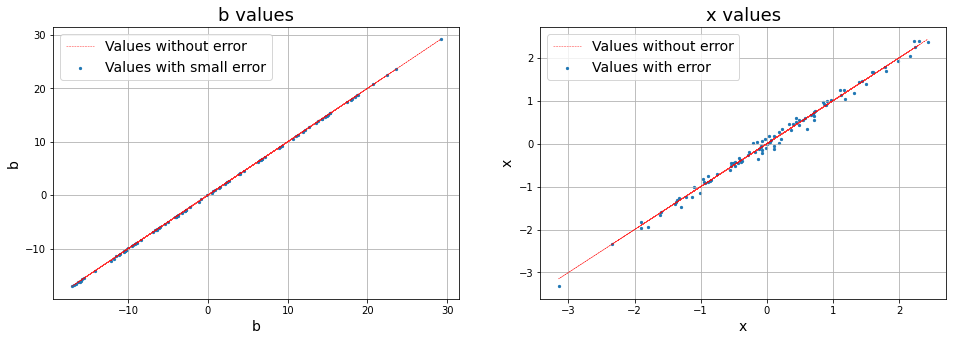
\includegraphics[width=1.0 \textwidth]{images/chapter2/ill_condition_demo.png}
	\caption{The influence of the condition number on the solution accuracy}
	\label{fig:ill_condition_demo}
\end{figure}